\documentclass{article}
\usepackage{amsmath}
\usepackage{multirow}
\usepackage{booktabs}
\usepackage{caption}
\usepackage{graphicx}
\usepackage{subcaption}

\DeclareMathOperator*{\argmax}{arg\,max}
\DeclareMathOperator*{\argmin}{arg\,min}

\usepackage{amsfonts}

\usepackage{tikz}
\usetikzlibrary{fit,positioning,shapes}

\usepackage[shortlabels]{enumitem}

\usepackage{algorithm}
\usepackage{amssymb}
\usepackage{booktabs}
\usepackage{algpseudocode}

\textwidth=7.6in
\textheight=9.9in
\topmargin=-.9in
\headheight=0in
\headsep=.5in
\hoffset=-1.5in
\setlength\parindent{0pt}


\begin{document}

\begin{center}
    \Large{\textbf{Problem Set 3 Solutions}} \\[0.25ex]
    Calvin Walker
\end{center}
\textbf{1.}
\begin{enumerate}[(a)]
    \item Consider the M-projection with the factored approximation $Q(X, Y) = Q(X)Q(Y)$, \begin{align*}
        D(P || Q) &= \sum_{X, Y} P(X, Y) \log \frac{P(X, Y)}{Q(X)Q(Y)} \\[0.5ex]
        &= \mathbb{E}_P[\log P(X, Y) - \log Q(X)Q(Y)] \\[0.5ex]
        &= \mathbb{E}_P[\log P(X, Y)] - \bigg(\mathbb{E}_p[\log Q(X)] + \mathbb{E}_p[\log Q(Y)]\bigg) \pm \log(P(X)P(Y)) \\[0.5ex]
        &= \mathbb{E}_p \bigg[\log \frac{P(X, Y)}{P(X)P(Y)}\bigg] + \mathbb{E}_p \bigg[\log \frac{P(X)}{Q(X)}\bigg] + \mathbb{E}_p \bigg[\log \frac{P(Y)}{Q(Y)}\bigg]
    \end{align*}
    Letting $Q^*_M = P(X)P(Y)$, \begin{align*}
        D(P || Q) &= D(P || Q^*_M) + \mathbb{E}_p \bigg[\log \frac{P(X)}{Q(X)}\bigg] + \mathbb{E}_p \bigg[\log \frac{P(Y)}{Q(Y)}\bigg]
    \end{align*}
    Thus, $D(P || Q) \geq D(P || Q^*_M)$, and $Q^*_M = P(X)P(Y)$ minimizes the M-projection. 
    \item \begin{align*}
        \theta^* &= \argmax_\theta \prod_{i = 1}^{M}Q(X^{(i)} ; \theta) \\[0.5ex]
        &= \argmin_\theta \sum_{i = 1}^{M} - \log Q(X^{(i)} ; \theta) \\[0.5ex]
        &= \argmin_\theta \sum_{i = 1}^{M} - \log Q(X^{(i)} ; \theta) + P(X^{(i)})
    \end{align*}
    So if the sample size $M$ is significantly large, \begin{align*}
        \theta^* &=  \argmin_\theta \ \mathbb{E}_P \bigg[\log \frac{P(X)}{Q(X ; \theta)} \bigg] \\[0.75ex]
        &= \argmin_\theta \ D(P || Q(X ; \theta))
    \end{align*}
    Therefore, the MLE solution $\theta^*$ minimizes the KL-Divergence $D(P || Q(X ; \theta))$, and is equivalent to solving for the M-projection $D(P||Q)$. 
    \item 
\end{enumerate}
\textbf{2.} 
\begin{enumerate}[(a)]
    \item $\mathcal{M} \subseteq Local[\mathcal{U}]$, since any valid distribution $P$ over $\mathcal{X}$ will satisfy the constraints of the local-consistency polytope. For a clique tree $\cal{T}$, under the constraints of the local-consistencey polytope, the pseudo marginals must be locally consistent, \begin{align*}
        \mu_{i,j}(S_{i,j}) = \sum_{C_i - S_{i,j}}\beta_i(C_i) = \sum_{C_j - S_{i,j}}\beta_i(C_j)
    \end{align*}
    which implies that the clique tree is calibrated. So we have the clique tree invariant \begin{align*}
        \Tilde{P}_{\Phi}(\mathcal{X}) = \frac{\prod_i \beta_i (C_i)}{\prod_{i,j} \mu_{i,j}(S_{i,j})}
    \end{align*} where $\beta_i(C_i) \propto \tilde{P}_{\Phi}(C_i)$ and $\mu_{i,j}(S_{i,j}) \propto \tilde{P}_{\Phi}(S_{i,j})$. Therefore, the clique and sepset marginals define a valid distribution over $\mathcal{X}$, and $Local[\mathcal{U}] \subseteq \mathcal{M}$. So we have that $Local[\mathcal{U}]$ is equivalent to $\cal{M}$ for a clique tree $\cal{T}$.
    
    \item \textcolor{white}{{x}}
    \begin{figure}[th]
        \centering
        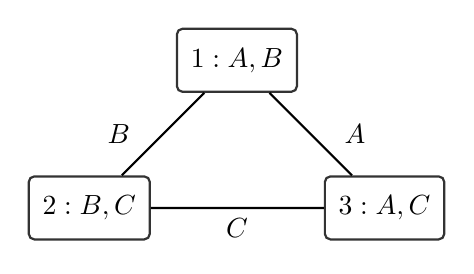
\begin{tikzpicture}[xscale=1.25,yscale=1.25]
            \tikzstyle{latent}=[rectangle, rounded corners=2pt, minimum size = 8mm, inner sep=5pt, thick, draw = black!80, node distance = 10mm]
            \tikzstyle{observed}=[rectangle, minimum size = 7mm, inner sep=0pt, thick, draw = black!80, node distance = 10mm,fill=gray!50]
            \tikzstyle{connect}=[thick]
            {\node[latent] (12) at (0,0.75){$1: A, B$};
            \node[latent] (23) at (-1.5,-0.75){$2: B, C$};
            \node[latent] (13) at (1.5,-0.75){$3: A, C$};
\node (x2) at (-1.2,0){$B$};
            \node (x3) at (0,-0.95){$C$};
            \node (x1) at (1.2,0){$A$};}
\path (12) edge [connect] (23);
            \path (23) edge [connect] (13);
            \path (13) edge [connect] (12);
        \end{tikzpicture}
        \caption{Example Cluster Graph}
        \label{fig:bethe-cluster-graph}
    \end{figure}

    Consider the above Cluster Graph for a pairwise MRF over three binary variables $A$, $B$, and $C$. We can satisfy the local consistency constraints with the following clique beliefs: 
\begin{gather*}
            \beta_{1}(A, B) =
            \begin{bmatrix}
                0.45 & 0.05\\ 0.05 & 0.45
            \end{bmatrix} \;
\beta_{2}(B, C) =
            \begin{bmatrix}
                0.45 & 0.05\\ 0.05 & 0.45
            \end{bmatrix}\;
\beta_{3}(A, C) =
            \begin{bmatrix}
                0.05 & 0.45 \\ 0.45 & 0.05
            \end{bmatrix}
    \end{gather*}
    Such that the sepset marginals are given by: $\mu_{1,3}(A) = \mu_{1,2}(B) = \mu_{2,3}(C) = (0.5, 0.5)$. If we assume that these are marginals for a valid probability distribution, 
    \begin{align*}
        P(A = 0, B = 0) = \beta_1(A = 0, B = 0) = 0.45 = P(0, 0, 1) + P(0, 0, 0) \\[0.5ex]
        P(A = 0, C = 0) = \beta_3(A = 0, C = 0) = 0.05 = P(0, 1, 0) + P(0, 0, 0) \\[0.5ex]
        P(B = 0, C = 1) = \beta_2(B = 0, C = 1) = 0.05 = P(1, 0, 1) + P(0, 0, 1)
    \end{align*}
    So $P(0, 0, 1) \leq 0.05$ and $P(0, 0, 0) \leq 0.05$, but $P(0, 0, 1) + P(0, 0, 0) = 0.45$.
    So the parameterization does not correspond to a valid probability distribution, and we can see for a cluster graph that is not a tree, the marginal polytope is strictly contained by the local consistency polytope. 
\end{enumerate}

\textbf{3.} \begin{enumerate}[(a)]
    \item \begin{enumerate}[(i)]
        \item We can see that the pseudo-marginal distributions satisfy the marginalization condition, since: \begin{align*}
            \mu_{1, 3}(X_1) = (0.5, 0.5) &= \sum_{X_2}\beta_1(X_1, X_2) = \sum_{X_3}\beta_3(X_1, X_3) \\[0.5ex]
            \mu_{1, 2}(X_2) = (0.5, 0.5) &= \sum_{X_1}\beta_1(X_1, X_2) = \sum_{X_3}\beta_2(X_2, X_3) \\[0.5ex]
            \mu_{2, 3}(X_3) = (0.5, 0.5) &= \sum_{X_2}\beta_2(X_2, X_3) = \sum_{X_1}\beta_3(X_1, X_3)
        \end{align*}
        And that the normalization conditions hold: \begin{align*}
            \sum_{X_1, X_2}\beta_1(X_1, X_2)  = \sum_{X_2, X_3}\beta_2(X_2, X_3) = \sum_{X_1, X_3}\beta_3(X_1, X_3) = 1
        \end{align*} and $\beta_i(c_i) \geq 0 \ \forall i $. Therefore, they are calibrated and locally consistent. 
        \item Assume that there is a valid distribution $P(X_1, X_2, X_3)$ with the beliefs as its marginals. Then, \begin{align*}
            P(X_1 = 0, X_2 = 0) = \beta_1(X_1 = 0, X_2 = 0) = 0.4 = P(0, 0, 1) + P(0, 0, 0) \\[0.5ex]
            P(X_1 = 0, X_3 = 0) = \beta_3(X_1 = 0, X_3 = 0) = 0.1 = P(0, 1, 0) + P(0, 0, 0) \\[0.5ex]
            P(X_2 = 0, X_3 = 1) = \beta_2(X_2 = 0, X_3 = 1) = 0.1 = P(1, 0, 1) + P(0, 0, 1)
        \end{align*}
        So $P(0, 0, 1) \leq 0.1$ and $P(0, 0, 0) \leq 0.1$, but $P(0, 0, 1) + P(0, 0, 0) = 0.4$, a contradiction. So the pseudo-marginals can't constitute a vaild distribution.
    \end{enumerate}
    \item \begin{align*}
        P_{\Phi}(A, B) - \beta_1(A, B) &= \sum_{C, D} P_{\Phi}(A, B, C, D) - \sum_{C, D} P_{\Phi}(A, B, C, D) r(A, D) \\
        &= P_{\Phi}(A, B) - P_{\Phi}(A, B) \sum_{D}r(A, D)
    \end{align*}
    So $\beta_1(A, B) =  P_{\Phi}(A, B) \sum_{D}r(A, D)$, and we have a bound on the error for the estimated marginal $\beta_1(A, B)$
\end{enumerate}
\textbf{4.} \begin{enumerate}[(a)]
    \item \textcolor{white}{{x}}
    \begin{table}[H]
        \centering
        \captionsetup{width=0.8\linewidth} % Adjust caption width
        \begin{minipage}[b]{0.45\linewidth}
            \centering
            \caption{GMM Mean Vectors (Foreground)}
            \begin{tabular}{@{}cccccc@{}}
                \toprule
                 1 & 2 & 3 & 4 & 5\\ \midrule
                 36.52 & 84.58 & 28.38 & 54.43 & 54.73\\
                 -0.13 & 17.19 & 10.62 & 22.38 & -1.72\\
                 -46.72 & 16.56 & -23.34 & 4.80 & -27.85\\ \bottomrule
            \end{tabular}
        \end{minipage}
        \hfill
        \begin{minipage}[b]{0.45\linewidth}
            \centering
            \caption{GMM Covariance Traces (Foreground)}
            \begin{tabular}{@{}ccccc@{}}
                \toprule
                1 & 2 & 3 & 4 & 5\\ \midrule
                7.05 & 35.98 & 44.74 & 131.42 & 108.44\\
                10.16 & 10.80 & 15.04 & 78.22 & 5.41 \\
                27.44 & 12.82 & 99.20 & 75.32 & 70.76\\ \bottomrule
            \end{tabular}
        \end{minipage}
    \end{table}
    \begin{table}[H]
        \centering
        \captionsetup{width=0.8\linewidth} % Adjust caption width
        \begin{minipage}[b]{0.45\linewidth}
            \centering
            \caption{GMM Mean Vectors (Background)}
            \begin{tabular}{@{}ccccc@{}}
                \toprule
                1 & 2 & 3 & 4 & 5 \\ \midrule
                87.89 & 67.91 & 44.28 & 97.85 & 75.99\\
                1.36 & 18.52 & 5.19 & 0.98 & -2.30 \\
                -3.51 & 13.05 & -9.32 & 0.89 & -11.15 \\ \bottomrule
            \end{tabular}
        \end{minipage}
        \hfill
        \begin{minipage}[b]{0.45\linewidth}
            \centering
            \caption{GMM Covariance Traces (Background)}
            \begin{tabular}{@{}ccccc@{}}
                \toprule
                1 & 2 & 3 & 4 & 5\\ \midrule
                19.86 & 6.27 & 25.90 & 0.18 & 67.36\\
                3.90 & 1.66 & 12.03 & 0.45 & 1.74 \\
                10.53 & 4.70 & 18.18 & 1.49 & 6.58 \\ \bottomrule
            \end{tabular}
        \end{minipage}
    \end{table}
\item \textcolor{white}{{x}} 
\begin{figure}[H]
    \centering
    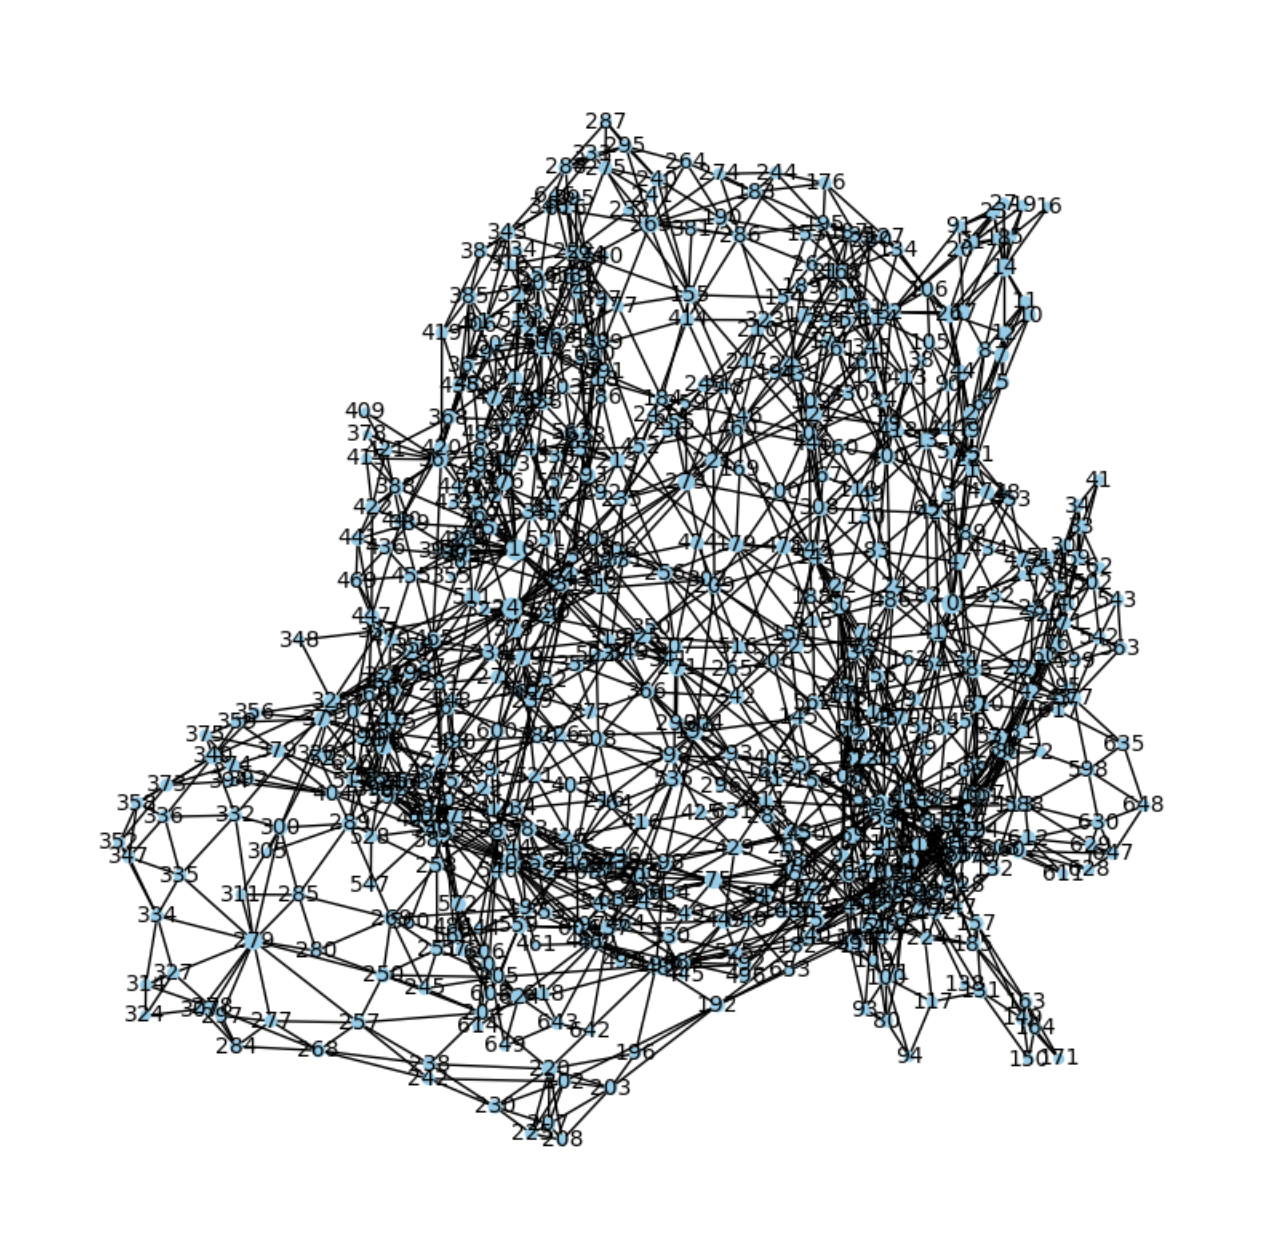
\includegraphics[scale=0.5]{adjmat.png}
    \caption{Visualization of Superpixel Adjacency Matrix}
\end{figure}
\item \textcolor{white}{{x}} 
\begin{figure}[H]
    \centering
    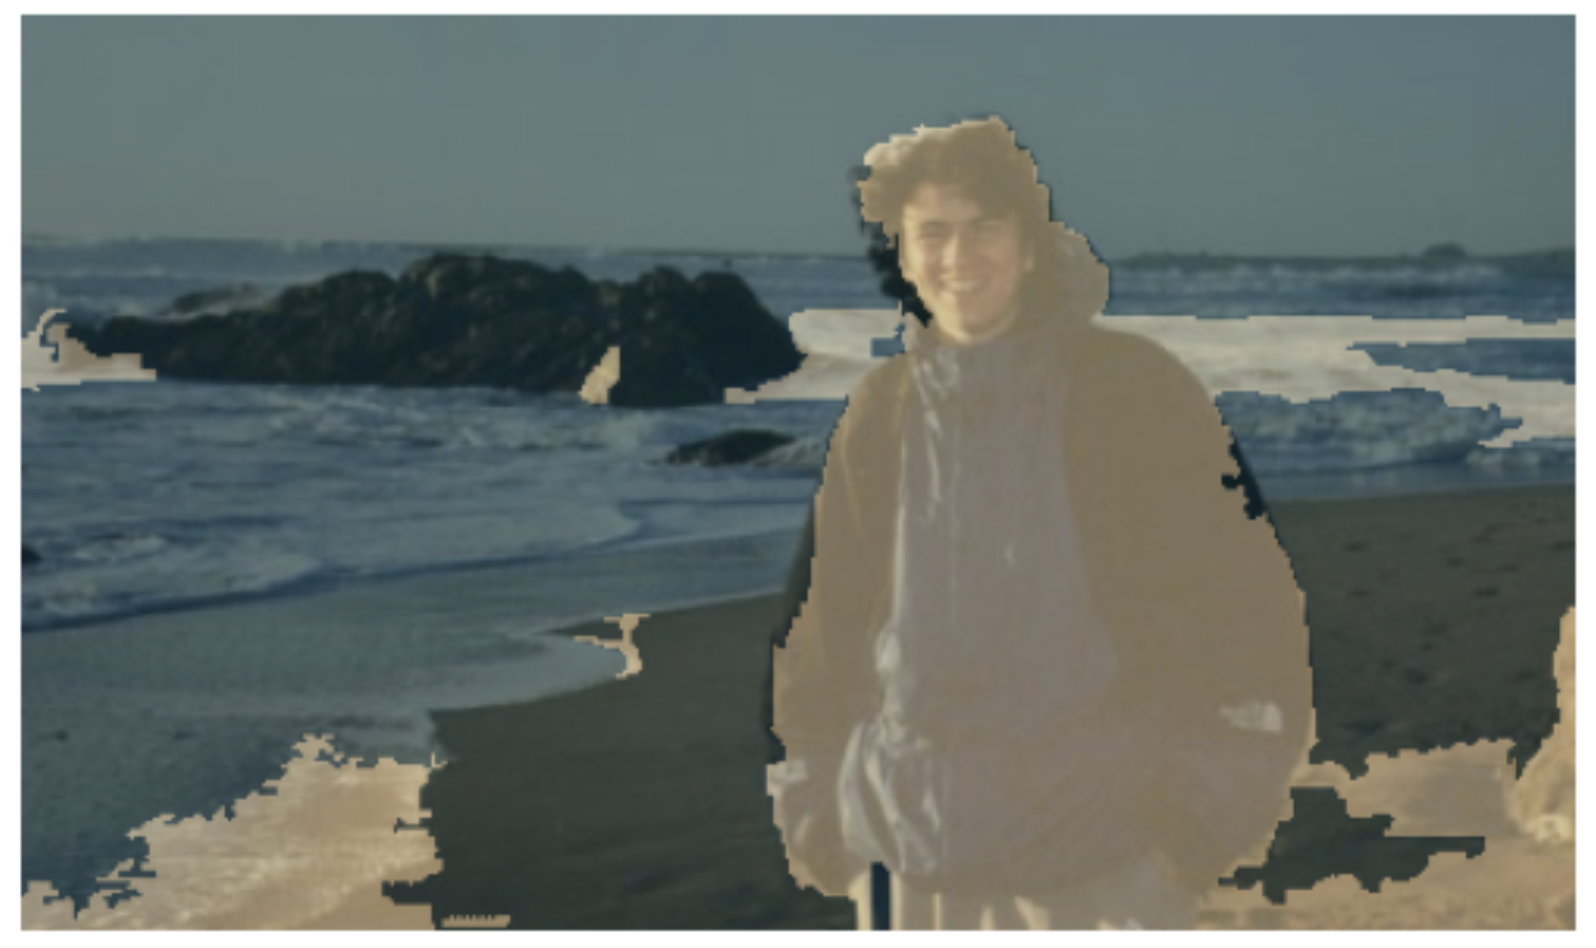
\includegraphics[scale=0.4]{beta2c.png}
    \caption{Result of Loopy Belief Propogation for $\beta = 2$}
\end{figure}
\item \textcolor{white}{{x}} 
\begin{figure}[H]
    \captionsetup[subfigure]{labelformat=empty}
    \centering
    \begin{subfigure}[b]{0.3\textwidth}
        \centering
        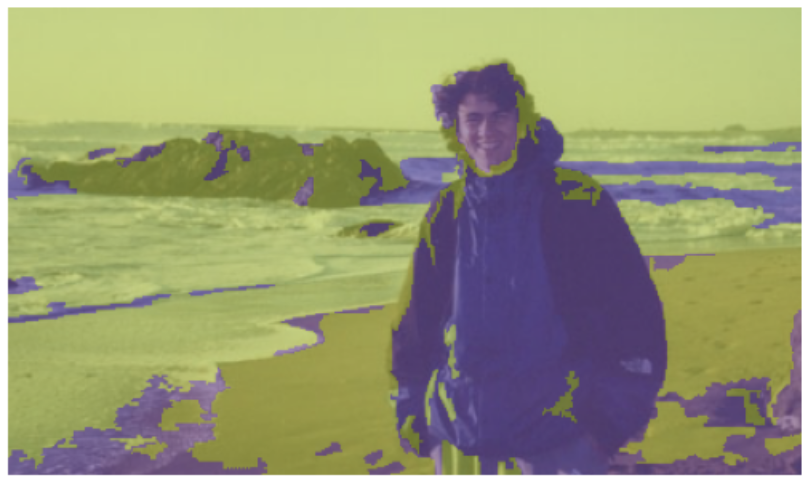
\includegraphics[width=\textwidth]{beta0.png}
        \caption{$\beta = 0$}
    \end{subfigure}
    \hfill
    \begin{subfigure}[b]{0.3\textwidth}
        \centering
        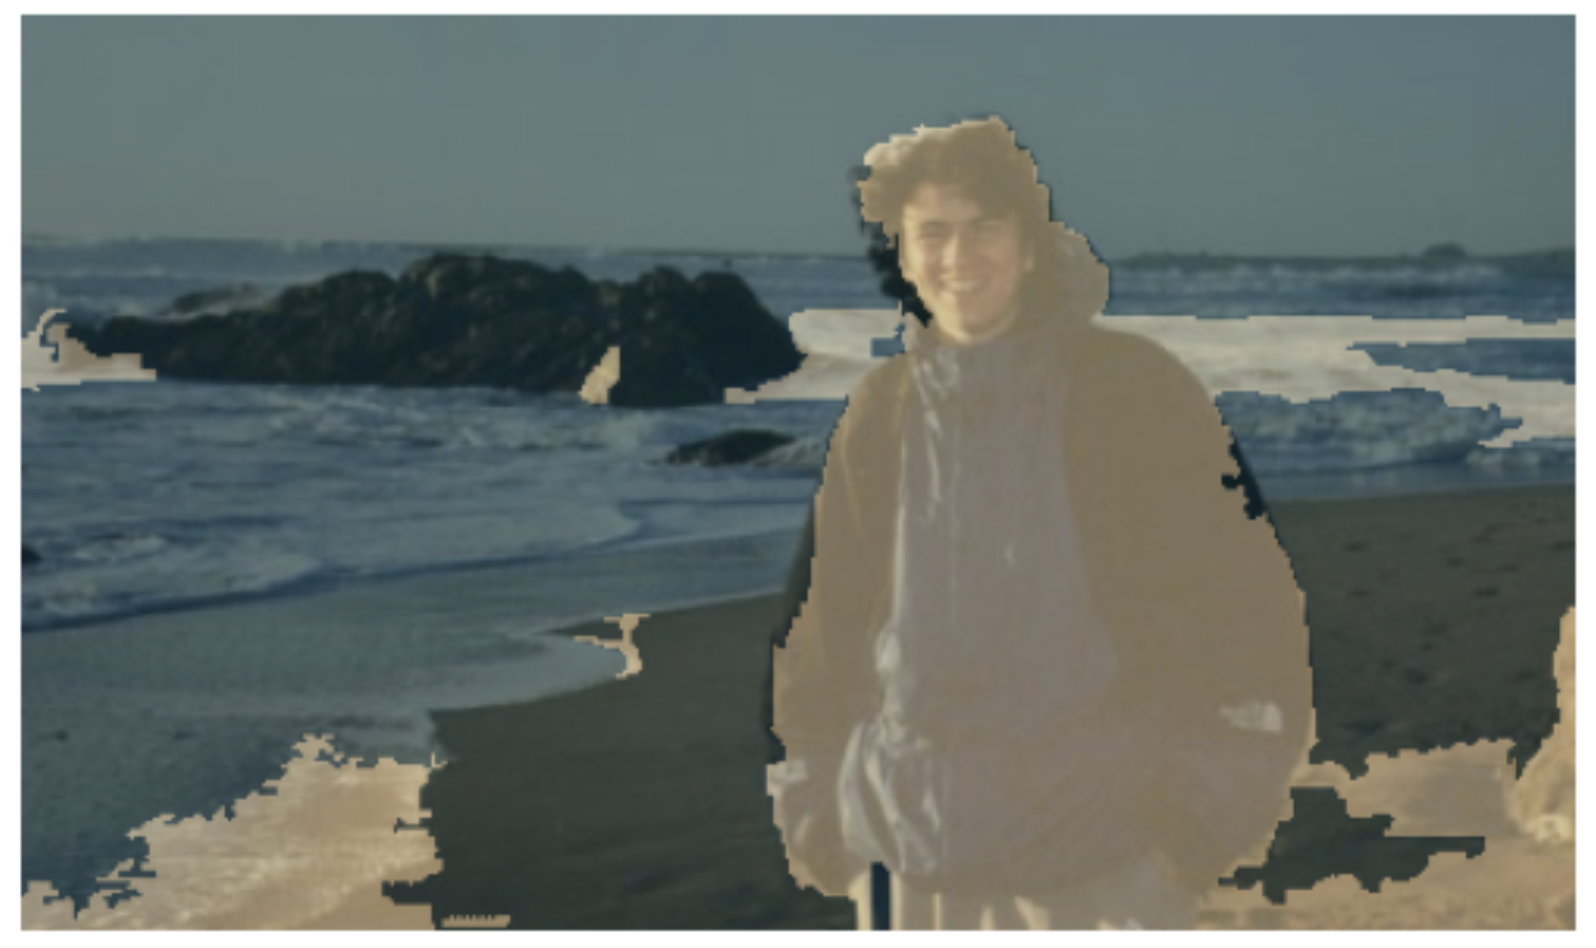
\includegraphics[width=\textwidth]{beta2c.png}
        \caption{$\beta = 2$}
    \end{subfigure}
    \hfill
    \begin{subfigure}[b]{0.3\textwidth}
        \centering
        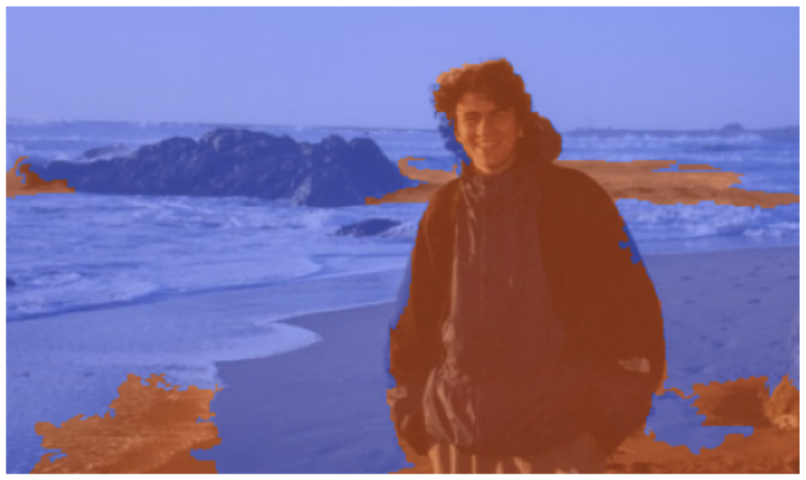
\includegraphics[width=\textwidth]{beta4.png}
        \caption{$\beta = 4$}
    \end{subfigure}
    \\
    \begin{subfigure}[b]{0.3\textwidth}
        \centering
        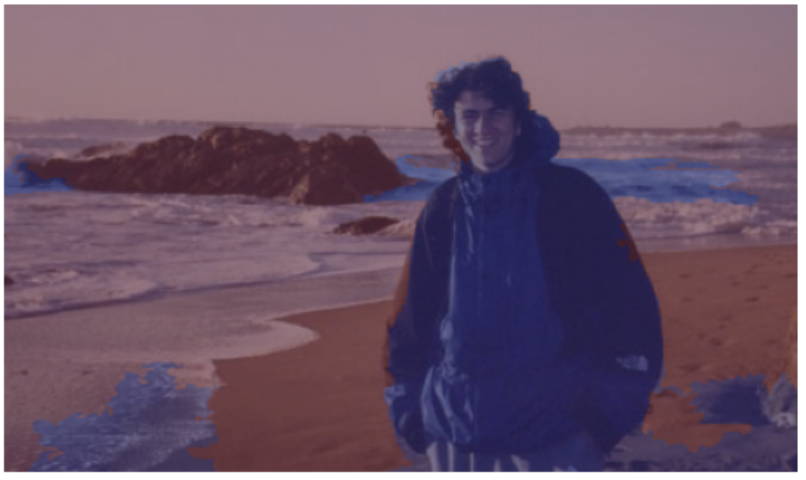
\includegraphics[width=\textwidth]{beta6.png}
        \caption{$\beta = 6$}
    \end{subfigure}
    \hfill
    \begin{subfigure}[b]{0.3\textwidth}
        \centering
        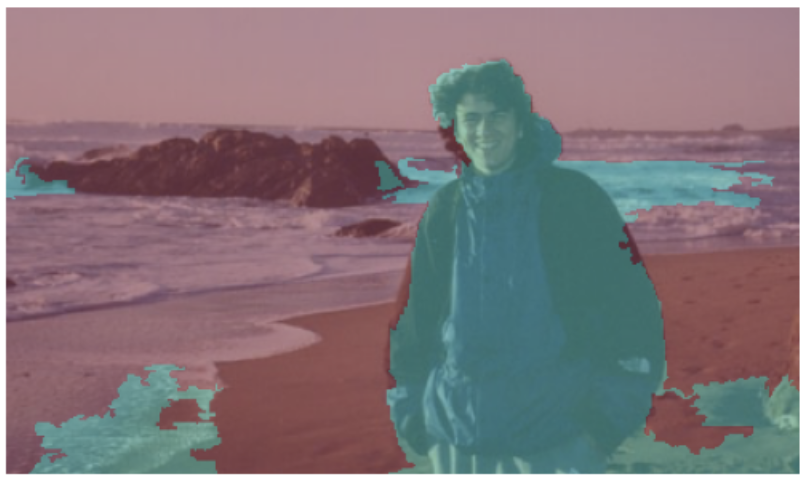
\includegraphics[width=\textwidth]{beta8.png}
        \caption{$\beta = 8$}
    \end{subfigure}
    \hfill
    \begin{subfigure}[b]{0.3\textwidth}
        \centering
        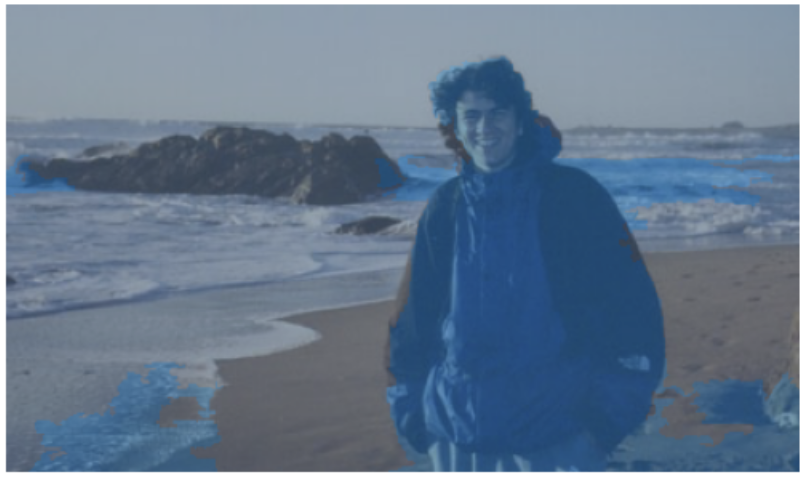
\includegraphics[width=\textwidth]{beta10.png}
        \caption{$\beta = 10$}
    \end{subfigure}
    \caption{Result of Loopy Belief Propogation for $\beta \in [0, 10]$}
    \label{fig:grid_of_images}
\end{figure}
$\beta = 0$ is special since all of the edge potentials are 1. The result of this is that there is less convergence between the different regions in the image, as we can see small areas with the background label even when the surrounding area is labeled foreground. As $\beta$ increaces, it appears that there is convergence towards larger continuous regions of the image with a single label. As $\beta \rightarrow \infty$, I would expect this behavior to continue, and the different labeled segments to converge, possibly until the entire image is labeled foreground or background.  
\end{enumerate}
\textbf{5.} \begin{enumerate}[(a)]
    \item I did not collaborate.
    \item 7 - 15 hours. 
\end{enumerate}

\end{document}